\documentclass[14pt]{extbook}
\usepackage{multicol, enumerate, enumitem, hyperref, color, soul, setspace, parskip, fancyhdr} %General Packages
\usepackage{amssymb, amsthm, amsmath, latexsym, units, mathtools} %Math Packages
\everymath{\displaystyle} %All math in Display Style
% Packages with additional options
\usepackage[headsep=0.5cm,headheight=12pt, left=1 in,right= 1 in,top= 1 in,bottom= 1 in]{geometry}
\usepackage[usenames,dvipsnames]{xcolor}
\usepackage{dashrule}  % Package to use the command below to create lines between items
\newcommand{\litem}[1]{\item#1\hspace*{-1cm}\rule{\textwidth}{0.4pt}}
\pagestyle{fancy}
\lhead{Progress Quiz 6}
\chead{}
\rhead{Version A}
\lfoot{4563-7456}
\cfoot{}
\rfoot{Summer C 2021}
\begin{document}

\begin{enumerate}
\litem{
Construct the lowest-degree polynomial given the zeros below. Then, choose the intervals that contain the coefficients of the polynomial in the form $x^3+bx^2+cx+d$.\[ -3 - 2 i \text{ and } -3 \]\begin{enumerate}[label=\Alph*.]
\item \( b \in [-5, 3], c \in [5.4, 6.45], \text{ and } d \in [7.9, 9.4] \)
\item \( b \in [-5, 3], c \in [4.58, 5.53], \text{ and } d \in [1.9, 7.1] \)
\item \( b \in [2, 13], c \in [30.15, 31.6], \text{ and } d \in [38.1, 39.8] \)
\item \( b \in [-17, -6], c \in [30.15, 31.6], \text{ and } d \in [-42, -38.7] \)
\item \( \text{None of the above.} \)

\end{enumerate} }
\litem{
Which of the following equations \textit{could} be of the graph presented below?
\begin{center}
    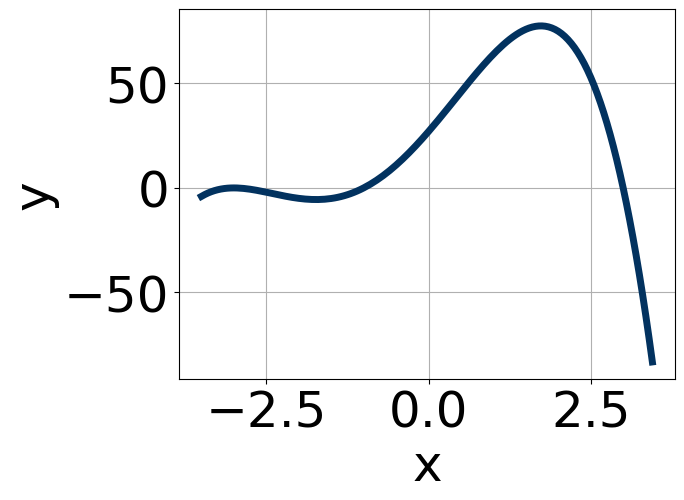
\includegraphics[width=0.5\textwidth]{../Figures/polyGraphToFunctionA.png}
\end{center}
\begin{enumerate}[label=\Alph*.]
\item \( -15(x + 3)^{10} (x - 3)^{7} (x + 1)^{11} \)
\item \( -9(x + 3)^{11} (x - 3)^{8} (x + 1)^{9} \)
\item \( -7(x + 3)^{10} (x - 3)^{6} (x + 1)^{7} \)
\item \( 5(x + 3)^{10} (x - 3)^{5} (x + 1)^{4} \)
\item \( 7(x + 3)^{6} (x - 3)^{5} (x + 1)^{5} \)

\end{enumerate} }
\litem{
Which of the following equations \textit{could} be of the graph presented below?
\begin{center}
    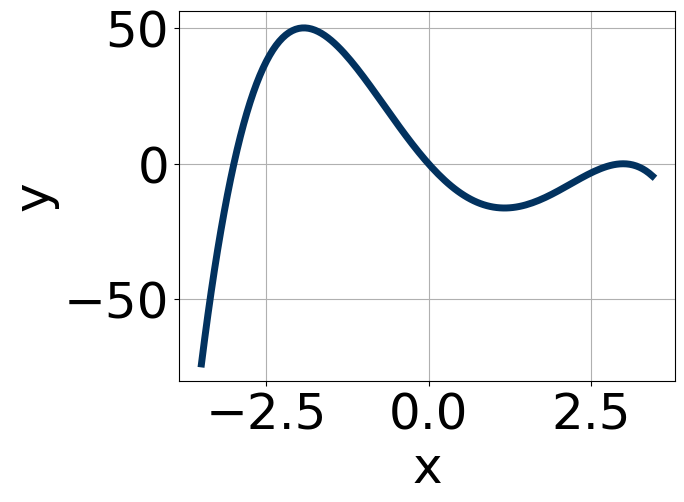
\includegraphics[width=0.5\textwidth]{../Figures/polyGraphToFunctionCopyA.png}
\end{center}
\begin{enumerate}[label=\Alph*.]
\item \( 10x^{7} (x - 3)^{4} (x + 3)^{10} \)
\item \( 15x^{11} (x - 3)^{6} (x + 3)^{5} \)
\item \( -20x^{6} (x - 3)^{9} (x + 3)^{7} \)
\item \( -7x^{7} (x - 3)^{8} (x + 3)^{5} \)
\item \( -18x^{4} (x - 3)^{4} (x + 3)^{5} \)

\end{enumerate} }
\litem{
Describe the zero behavior of the zero $x = 4$ of the polynomial below.\[ f(x) = 2(x + 6)^{8}(x - 6)^{4}(x - 4)^{10}(x + 4)^{7} \]\begin{enumerate}[label=\Alph*.]
\begin{multicols}{2}\item 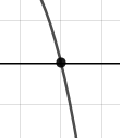
\includegraphics[width = 0.3\textwidth]{../Figures/polyZeroBehaviorCopyAA.png}\item 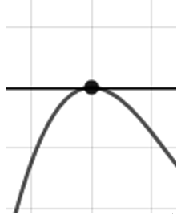
\includegraphics[width = 0.3\textwidth]{../Figures/polyZeroBehaviorCopyBA.png}\item 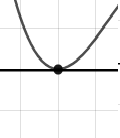
\includegraphics[width = 0.3\textwidth]{../Figures/polyZeroBehaviorCopyCA.png}\item 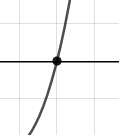
\includegraphics[width = 0.3\textwidth]{../Figures/polyZeroBehaviorCopyDA.png}\end{multicols}\item None of the above.
\end{enumerate} }
\litem{
Construct the lowest-degree polynomial given the zeros below. Then, choose the intervals that contain the coefficients of the polynomial in the form $x^3+bx^2+cx+d$.\[ 2 + 3 i \text{ and } 3 \]\begin{enumerate}[label=\Alph*.]
\item \( b \in [4, 11], c \in [21.54, 25.63], \text{ and } d \in [33, 43] \)
\item \( b \in [-3, 5], c \in [-5.17, -2.87], \text{ and } d \in [0, 7] \)
\item \( b \in [-3, 5], c \in [-6.83, -5.89], \text{ and } d \in [9, 10] \)
\item \( b \in [-9, -4], c \in [21.54, 25.63], \text{ and } d \in [-46, -38] \)
\item \( \text{None of the above.} \)

\end{enumerate} }
\litem{
Construct the lowest-degree polynomial given the zeros below. Then, choose the intervals that contain the coefficients of the polynomial in the form $ax^3+bx^2+cx+d$.\[ \frac{3}{5}, \frac{-1}{3}, \text{ and } \frac{-1}{2} \]\begin{enumerate}[label=\Alph*.]
\item \( a \in [30, 39], b \in [-13, -1], c \in [-13, -6], \text{ and } d \in [-1, 7] \)
\item \( a \in [30, 39], b \in [40, 44], c \in [18, 24], \text{ and } d \in [-1, 7] \)
\item \( a \in [30, 39], b \in [22, 27], c \in [-2, 0], \text{ and } d \in [-3, -2] \)
\item \( a \in [30, 39], b \in [7, 13], c \in [-13, -6], \text{ and } d \in [-1, 7] \)
\item \( a \in [30, 39], b \in [7, 13], c \in [-13, -6], \text{ and } d \in [-3, -2] \)

\end{enumerate} }
\litem{
Describe the end behavior of the polynomial below.\[ f(x) = -7(x - 9)^{5}(x + 9)^{8}(x + 4)^{5}(x - 4)^{7} \]\begin{enumerate}[label=\Alph*.]
\begin{multicols}{2}\item 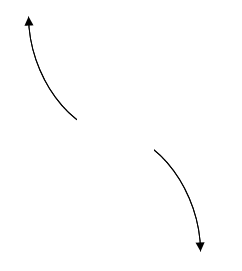
\includegraphics[width = 0.3\textwidth]{../Figures/polyEndBehaviorAA.png}\item 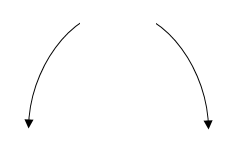
\includegraphics[width = 0.3\textwidth]{../Figures/polyEndBehaviorBA.png}\item 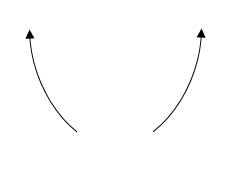
\includegraphics[width = 0.3\textwidth]{../Figures/polyEndBehaviorCA.png}\item 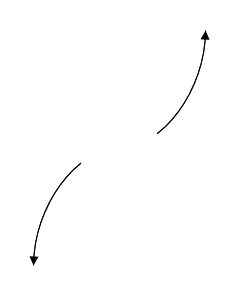
\includegraphics[width = 0.3\textwidth]{../Figures/polyEndBehaviorDA.png}\end{multicols}\item None of the above.
\end{enumerate} }
\litem{
Construct the lowest-degree polynomial given the zeros below. Then, choose the intervals that contain the coefficients of the polynomial in the form $ax^3+bx^2+cx+d$.\[ \frac{-6}{5}, \frac{3}{5}, \text{ and } \frac{7}{2} \]\begin{enumerate}[label=\Alph*.]
\item \( a \in [48, 54], b \in [-154, -139], c \in [-141, -135], \text{ and } d \in [-128, -118] \)
\item \( a \in [48, 54], b \in [-206, -201], c \in [67, 73], \text{ and } d \in [125, 132] \)
\item \( a \in [48, 54], b \in [-267, -261], c \in [350, 357], \text{ and } d \in [-128, -118] \)
\item \( a \in [48, 54], b \in [142, 152], c \in [-141, -135], \text{ and } d \in [-128, -118] \)
\item \( a \in [48, 54], b \in [-154, -139], c \in [-141, -135], \text{ and } d \in [125, 132] \)

\end{enumerate} }
\litem{
Describe the zero behavior of the zero $x = 5$ of the polynomial below.\[ f(x) = -7(x - 3)^{6}(x + 3)^{3}(x - 5)^{10}(x + 5)^{7} \]\begin{enumerate}[label=\Alph*.]
\begin{multicols}{2}\item 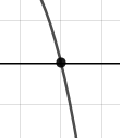
\includegraphics[width = 0.3\textwidth]{../Figures/polyZeroBehaviorAA.png}\item 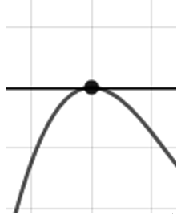
\includegraphics[width = 0.3\textwidth]{../Figures/polyZeroBehaviorBA.png}\item 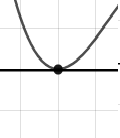
\includegraphics[width = 0.3\textwidth]{../Figures/polyZeroBehaviorCA.png}\item 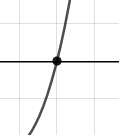
\includegraphics[width = 0.3\textwidth]{../Figures/polyZeroBehaviorDA.png}\end{multicols}\item None of the above.
\end{enumerate} }
\litem{
Describe the end behavior of the polynomial below.\[ f(x) = -8(x + 3)^{4}(x - 3)^{5}(x + 7)^{3}(x - 7)^{5} \]\begin{enumerate}[label=\Alph*.]
\begin{multicols}{2}\item 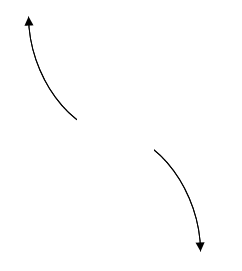
\includegraphics[width = 0.3\textwidth]{../Figures/polyEndBehaviorCopyAA.png}\item 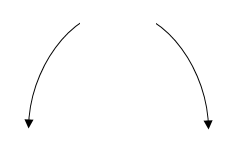
\includegraphics[width = 0.3\textwidth]{../Figures/polyEndBehaviorCopyBA.png}\item 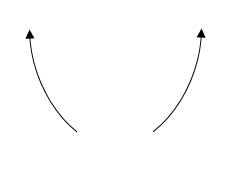
\includegraphics[width = 0.3\textwidth]{../Figures/polyEndBehaviorCopyCA.png}\item 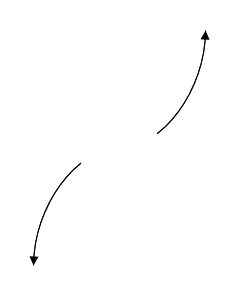
\includegraphics[width = 0.3\textwidth]{../Figures/polyEndBehaviorCopyDA.png}\end{multicols}\item None of the above.
\end{enumerate} }
\end{enumerate}

\end{document}